\documentclass[aspectratio=169]{beamer}

\usefonttheme[onlymath]{serif}

\usepackage{physics}
\usepackage[export]{adjustbox}
\usepackage[absolute,overlay]{textpos}
\usepackage{graphicx}

\usepackage{derivative}
% I should not have to do this
\DeclareOdvVariant{\odv}{d}[style-inf=\mathrm] 


% \title{Kiral perturbasjonsteori}

\author{Martin Johnsrud}

\begin{document}
    % \frame{\titlepage}

    \begin{frame}
        \frametitle{Pion stars}
        \begin{itemize}
            \itemsep 0.4cm
            \item New proposal: stars made of pions
            \item Microscopic part: what are the\\ thermodynamics of pions?
            \item Macroscopic part: hydrodynamics of\\
             astrophysical objects
            \item Questions: What is the mass-radius relations of pion stars?
            How do EM-interactions/including three quarks/loop corrections influence the star?
        \end{itemize}

        \begin{textblock}{8}(8, 1)
            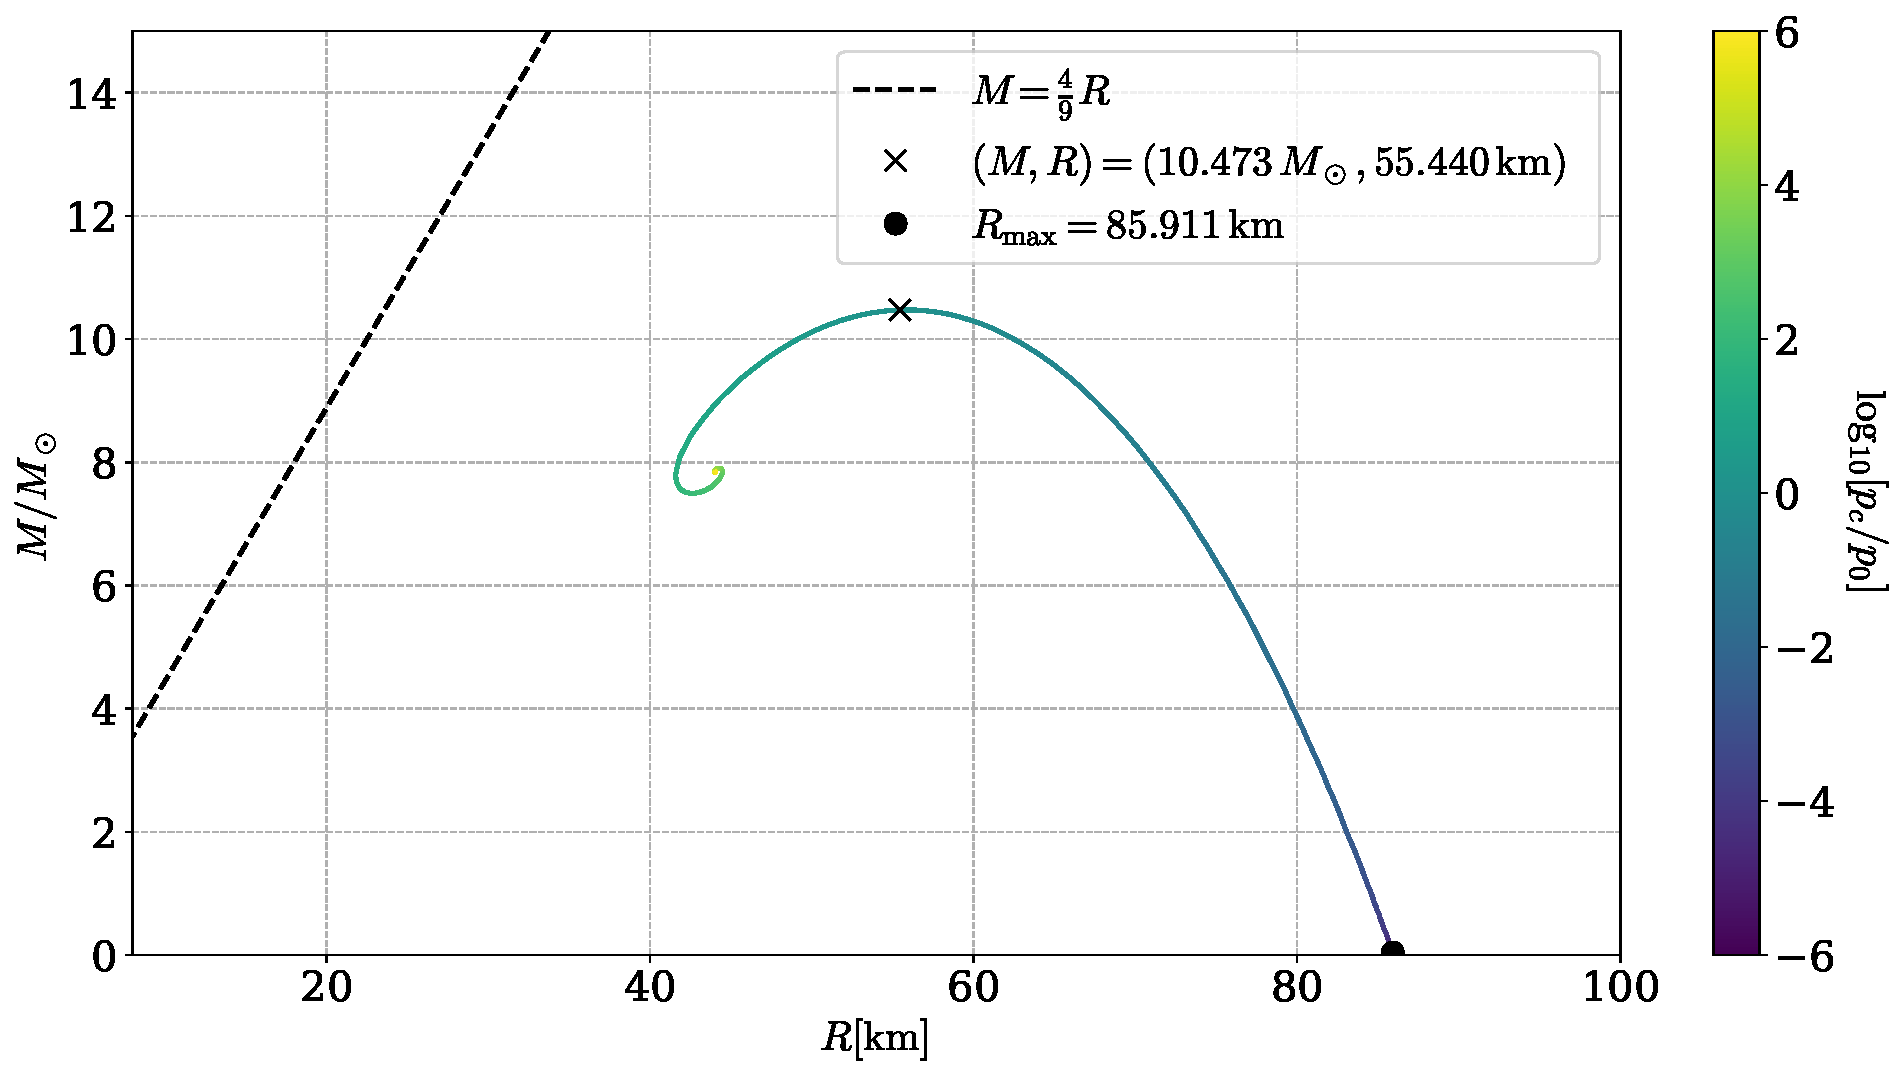
\includegraphics[width=\textwidth]{../../scripts/figurer/pion_star/mass_radius_pion_star.pdf}
        \end{textblock}


    \end{frame}

    \begin{frame}

        \frametitle{Chiral perturbation theory}

        \begin{textblock}{4.8}(10.5, 2)
            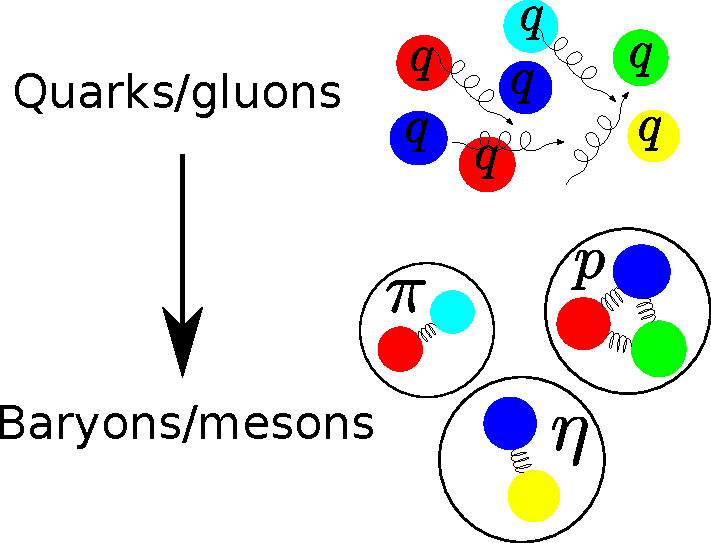
\includegraphics[width=\textwidth]{quarks-to-mesons.pdf}
        \end{textblock}

        \begin{itemize}
            \itemsep 0.4cm
            \item Quarks bind into baryon (protons/neutrons) and \\ mesons (pions) at low temperatures ($< \, \sim10^{12}$ K)
            \item The strong force is strong, so we can't do\\ perturbation theory.\\
            $
            \mathcal L = 
            \sum_f \bar q_f (\gamma^\mu [\partial_\mu - i q \lambda^a A^a_\mu ] + m_f)q_f
            + G^a_{\mu \nu} G_a^{\mu \nu}
            $
            \item Need an effective theory, The QCD vacuum spontaneously break a symmetry of the Lagrangian --- Goldstone bosons (pions)\\
            $
            \mathcal L_\text{eff} = 
            \frac{f^2}{4} \Tr{\nabla_\mu \Sigma \nabla^\mu \Sigma^\dagger}
            + \frac{f^2}{4} \Tr{\chi^\dagger \Sigma + \Sigma^\dagger \chi} 
            + l_1 \Tr{\nabla_\mu \Sigma (\nabla^\mu \Sigma)^\dagger}^2+
            \dots
            $ \\
            \item $\Sigma = \exp\left( i \pi_a \tau_a / f \right) \in \text{SU}(3)$, where $\text{SU}(3)$ is the broken symmetry.

        \end{itemize}


    \end{frame}

    \begin{frame}
        \frametitle{Thermodynamics}

        \begin{textblock}{7}(8.5, 7)
            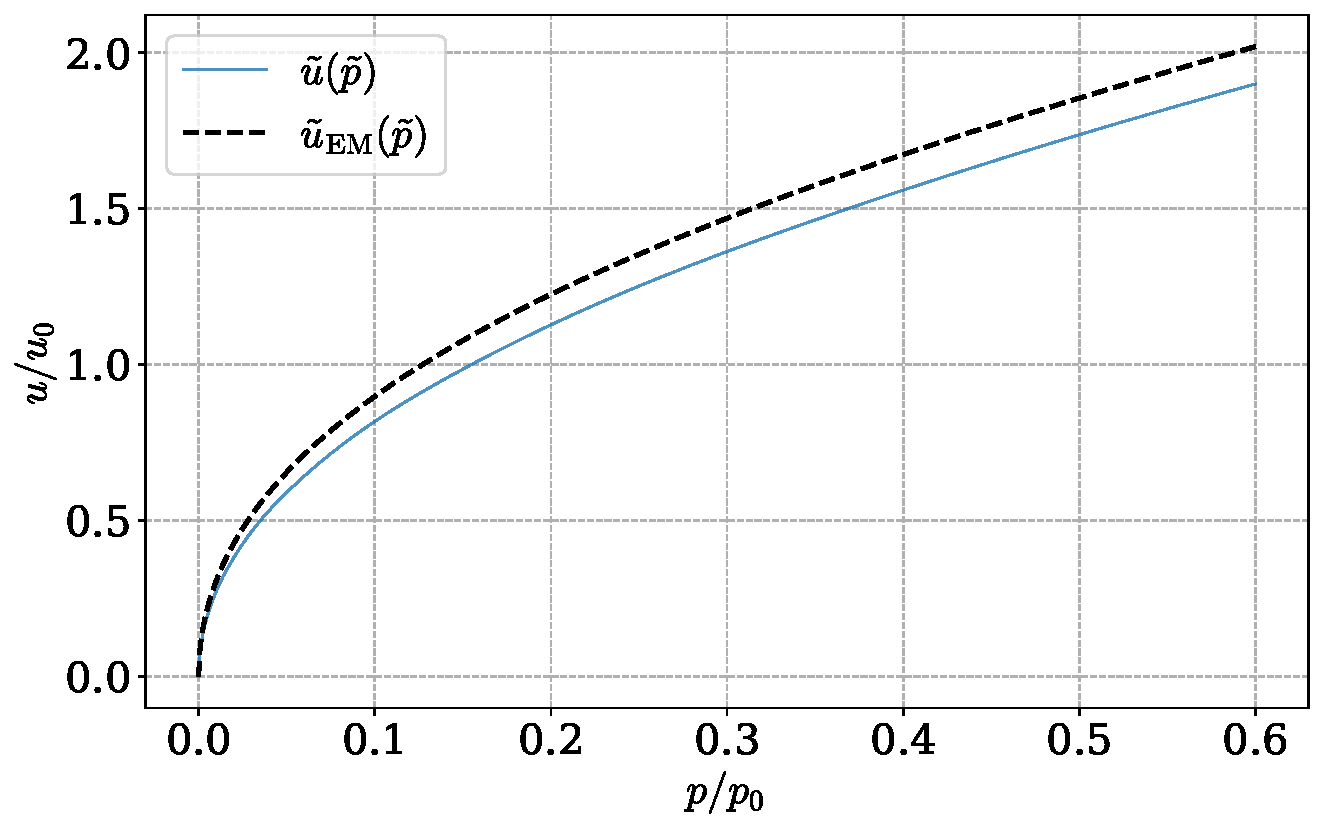
\includegraphics[width=\textwidth]{../../scripts/figurer/pion_star/pion_eos_EM.pdf}
        \end{textblock}
         
        \begin{itemize}
            \itemsep 0.4cm
            \item With the effective Lagrangian, we can calculate free energy density
            \item $
            \mathcal{F}
            = -\frac{i}{V \beta} 
            \ln\left[
                 \int \mathcal D \pi \, \exp
                 \left(
                    i \int \dd^4x \, [\mathcal{L}_\text{eff} + \mu J]
                 \right)
            \right]
            $
            \item Include isospin and strangeness chemical \\
            potential, EM-interactions, loops...
            \item Phase transitions: pion condensation
            \item Calculate equation of state
        \end{itemize}
    \end{frame}

    \begin{frame}
        \frametitle{Hydrostatic equilibrium}

        \begin{columns}
        \begin{column}{0.4\textwidth}


        \begin{itemize}
            \itemsep 0.6cm
            \item TOV equation govern pressure of perfect fluids in hydrostatic equilibrium\\
            $
            \odv{P}{r} = - \frac{G}{r^2} 
            \frac{\left(u + P\right)
            \left(m + 4 \pi r^3 P\right)}
            {\left(1 - \frac{2Gm}{r} \right)}
            ,
            $ \\
            $
            \odv{m}{r} = 4 \pi r^2 u
            $
            \item Numerical integration gives $P$, $u$ and thus $M$, $R$. 
        \end{itemize}

        \end{column}
        \begin{column}{0.6\textwidth}
            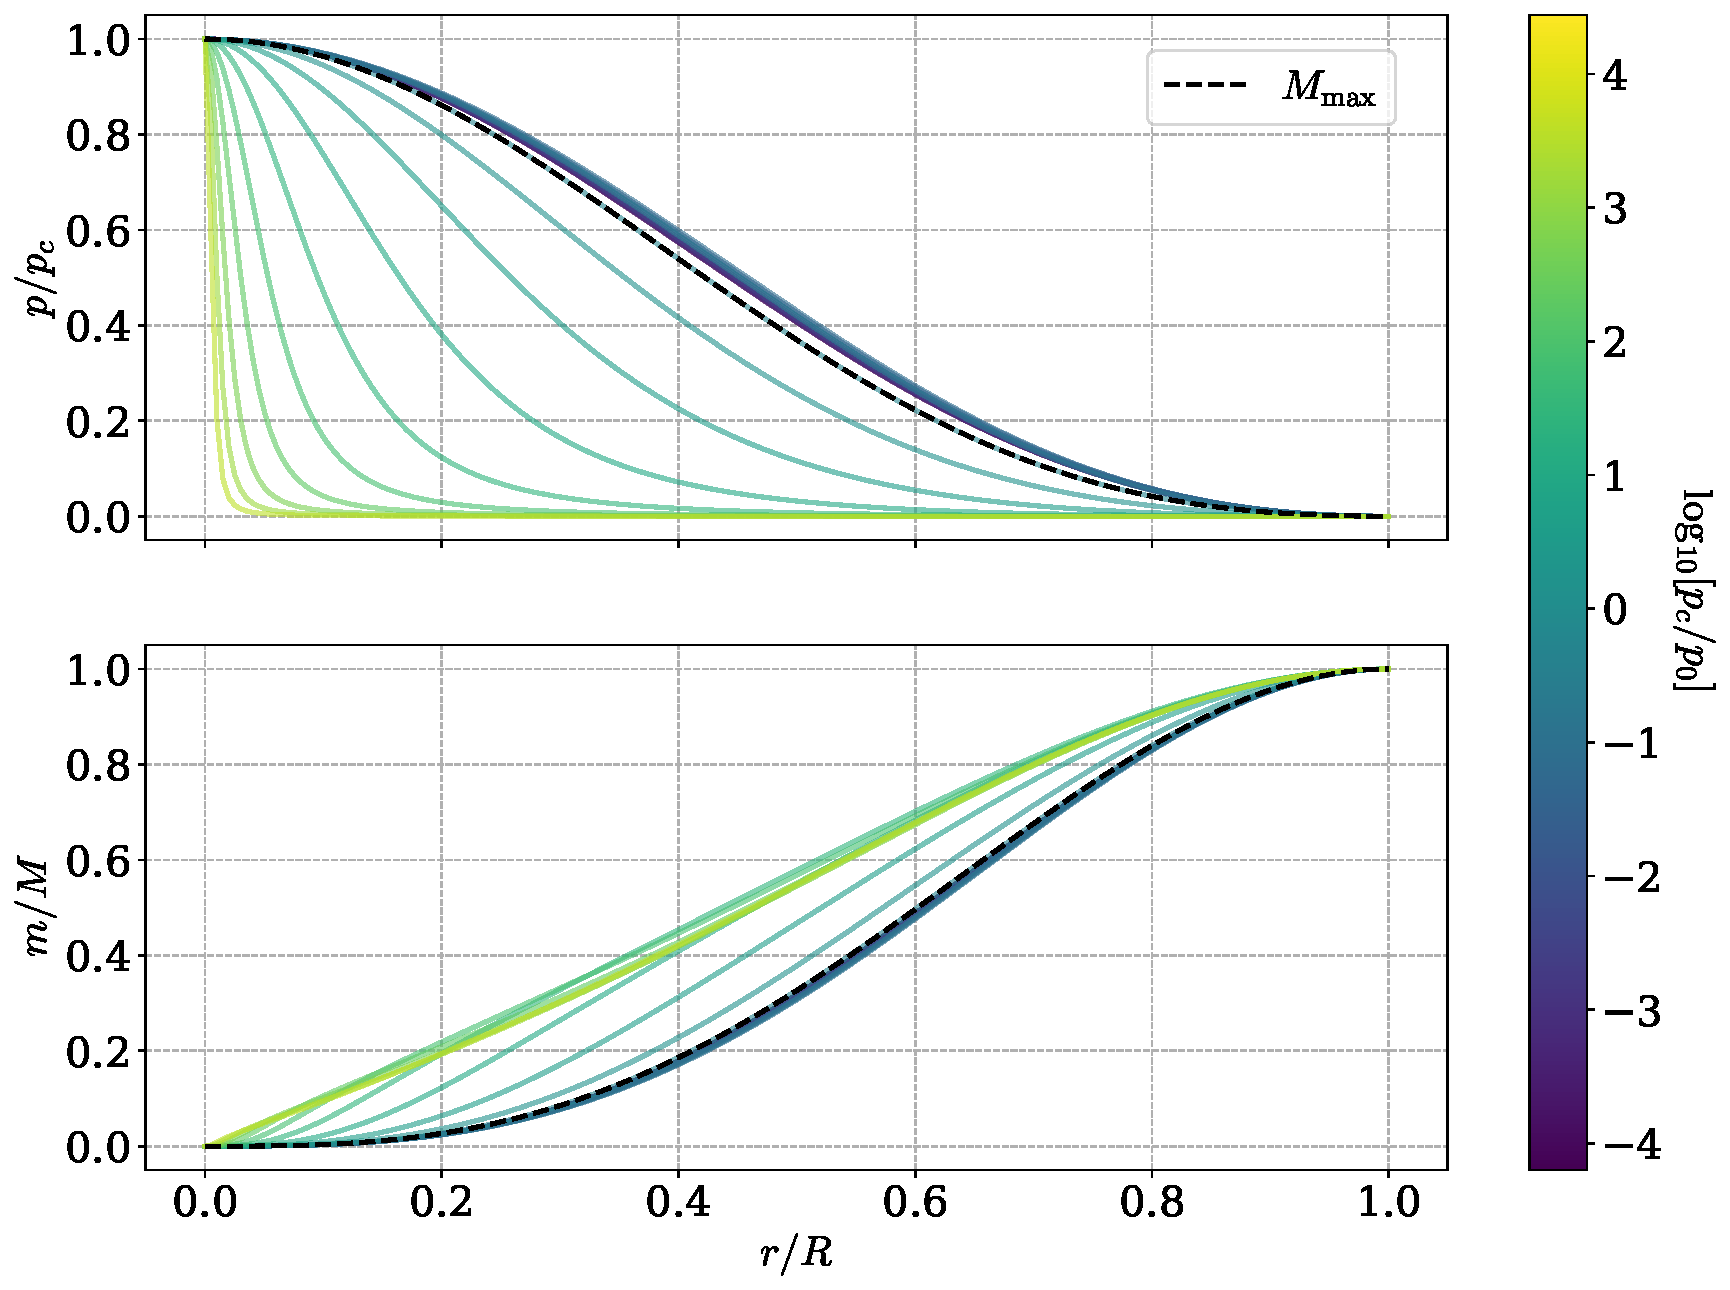
\includegraphics[width=\textwidth]{../../scripts/figurer/pion_star/pressure_mass_pion_star.pdf}
        \end{column}
        \end{columns}
    \end{frame}

    \begin{frame}
        \frametitle{Results}
        We get a family of results parametrized by central pressure.
        \vspace{1cm}
        \begin{columns}
            \begin{column}{0.55\textwidth}
                Neutron star
                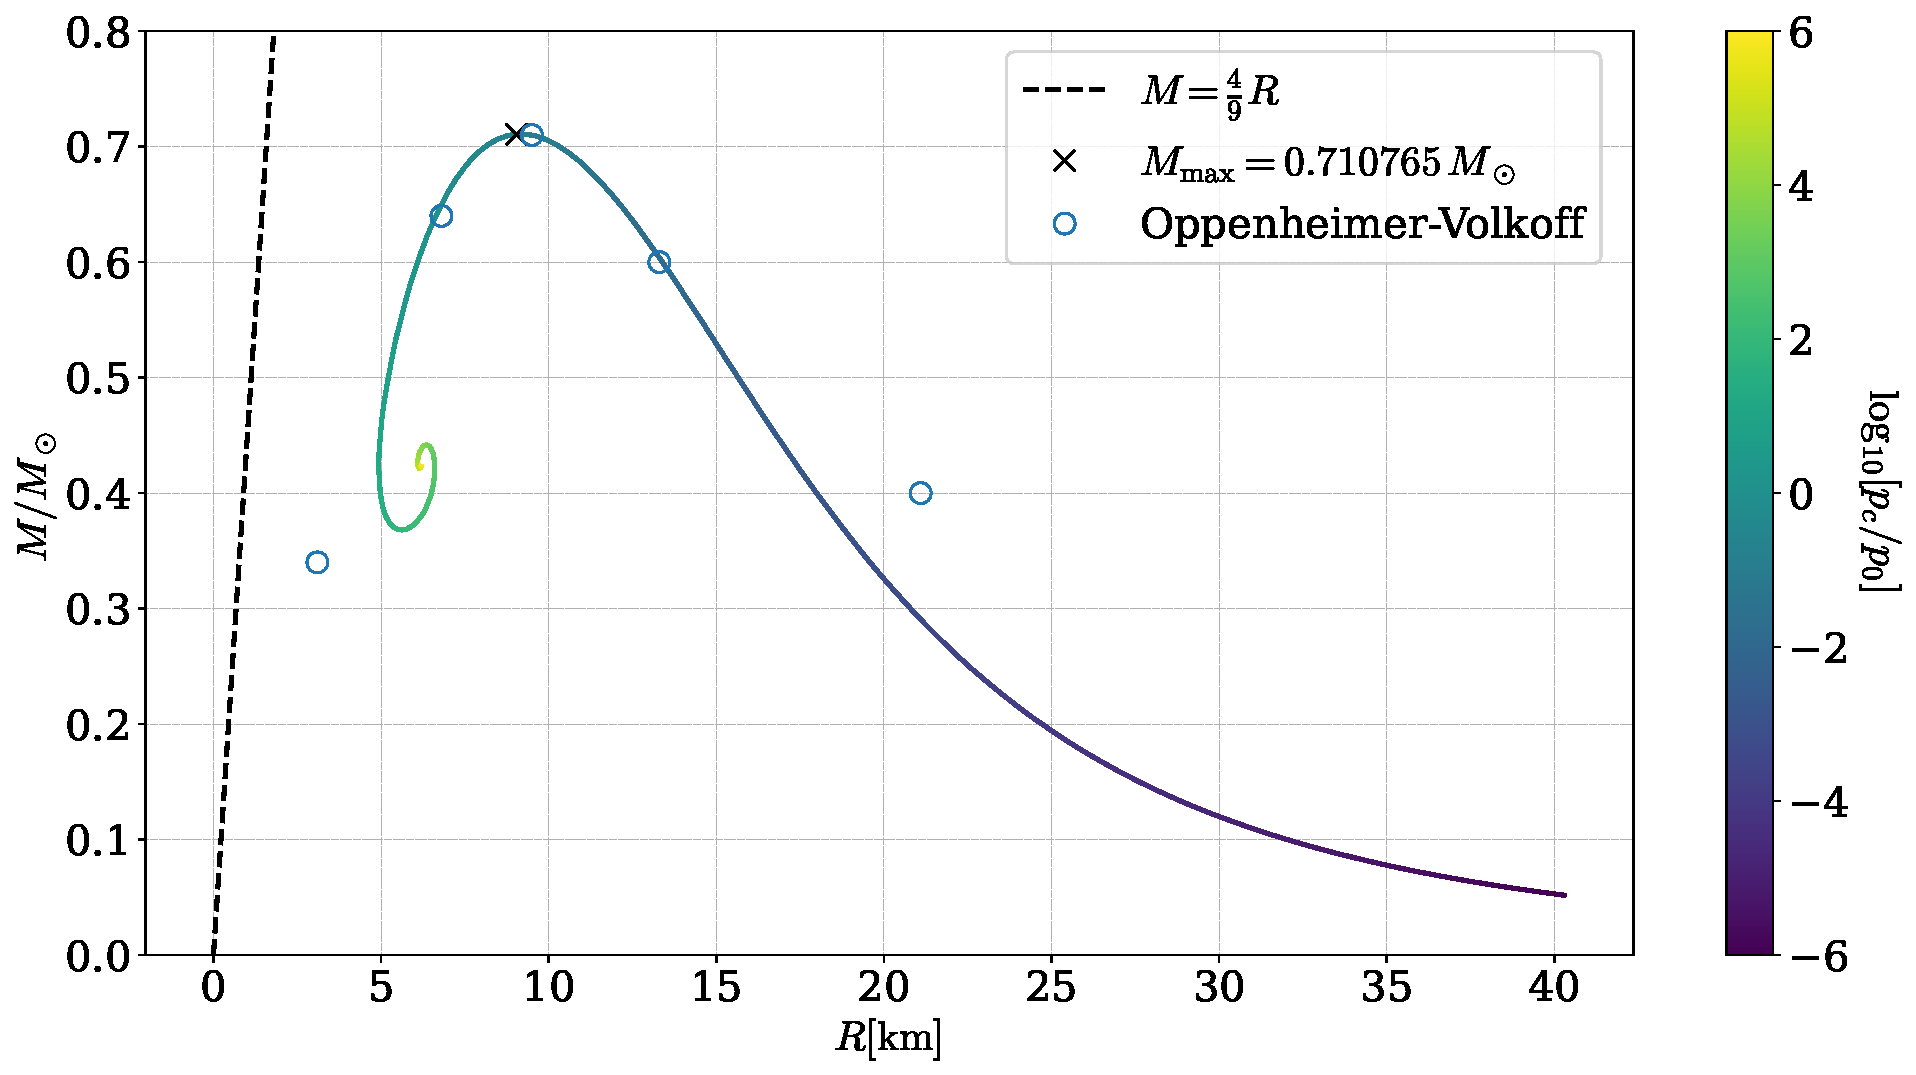
\includegraphics[width=\textwidth]{../../scripts/figurer/mass_radius_neutron.pdf}
            \end{column}
            \begin{column}{0.55\textwidth}
                Pion star
                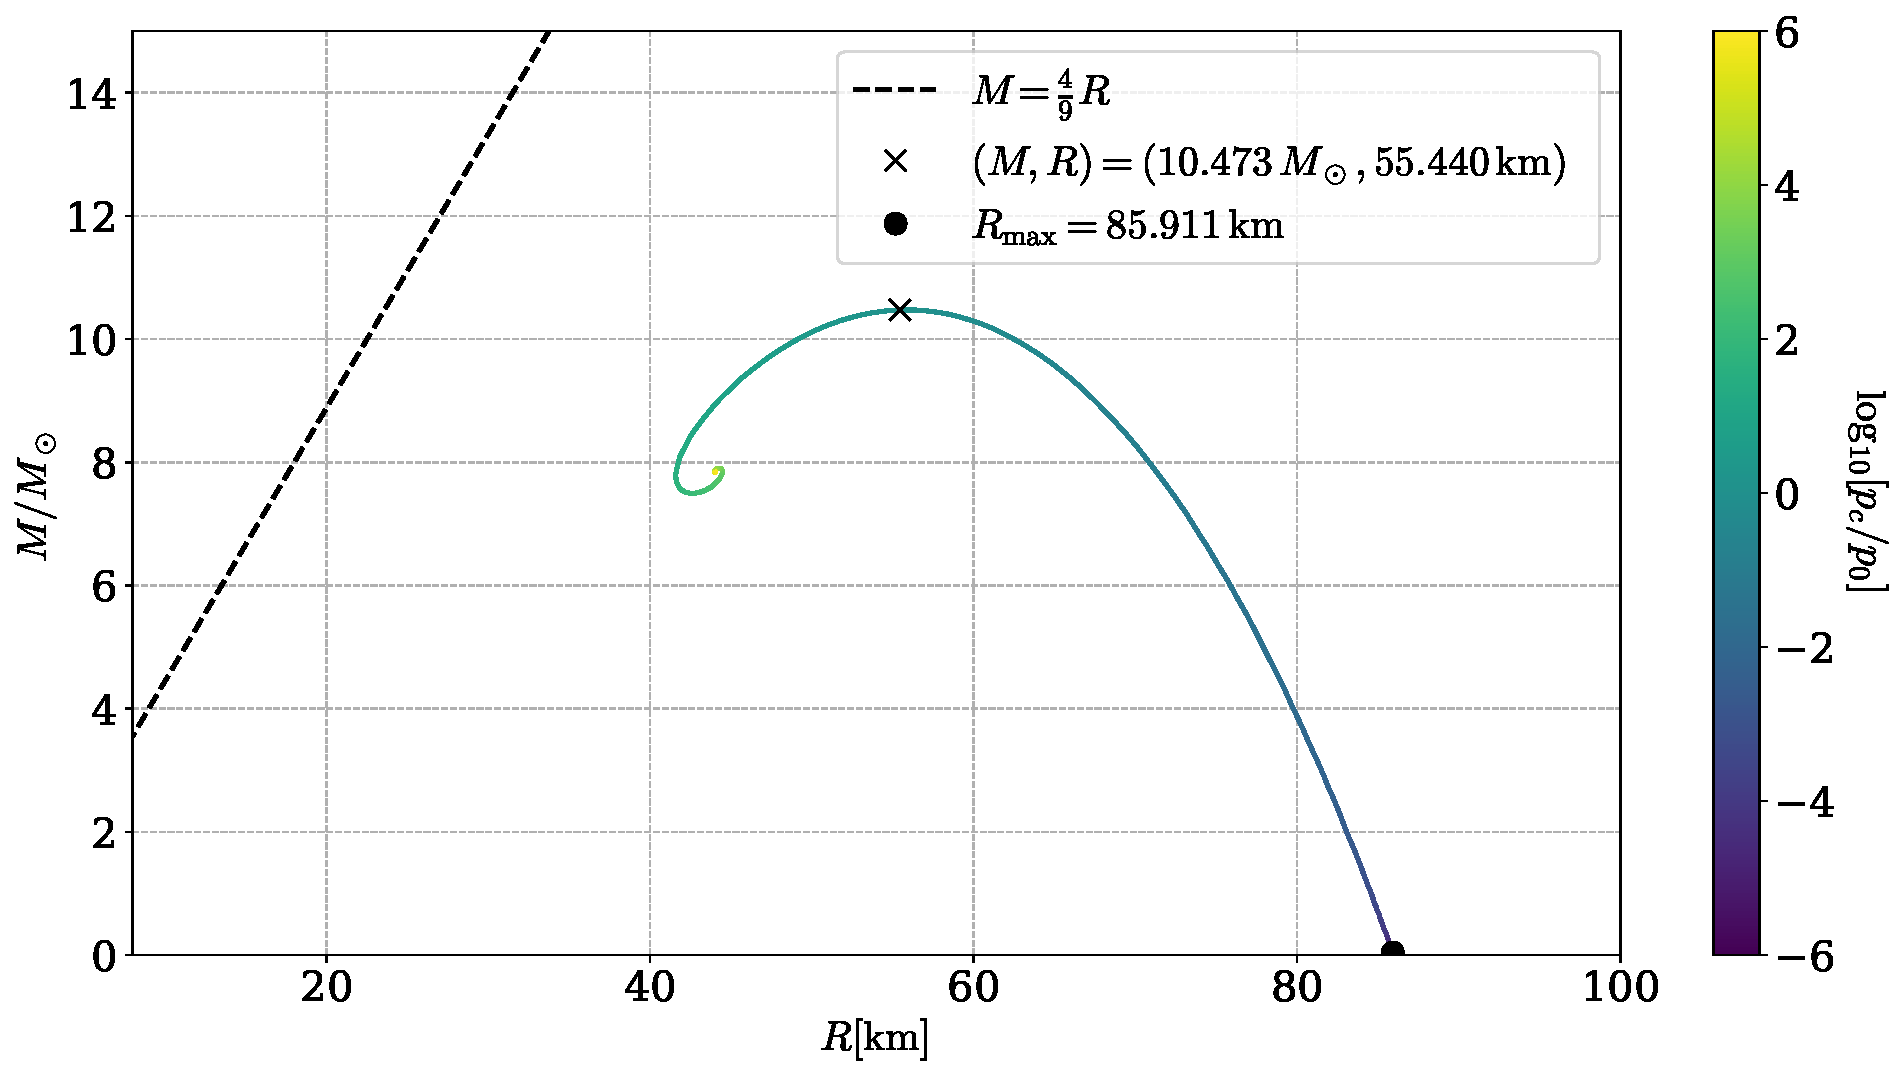
\includegraphics[width=\textwidth]{../../scripts/figurer/pion_star/mass_radius_pion_star.pdf}
            \end{column}
        \end{columns}
    \end{frame}

    \begin{frame}
        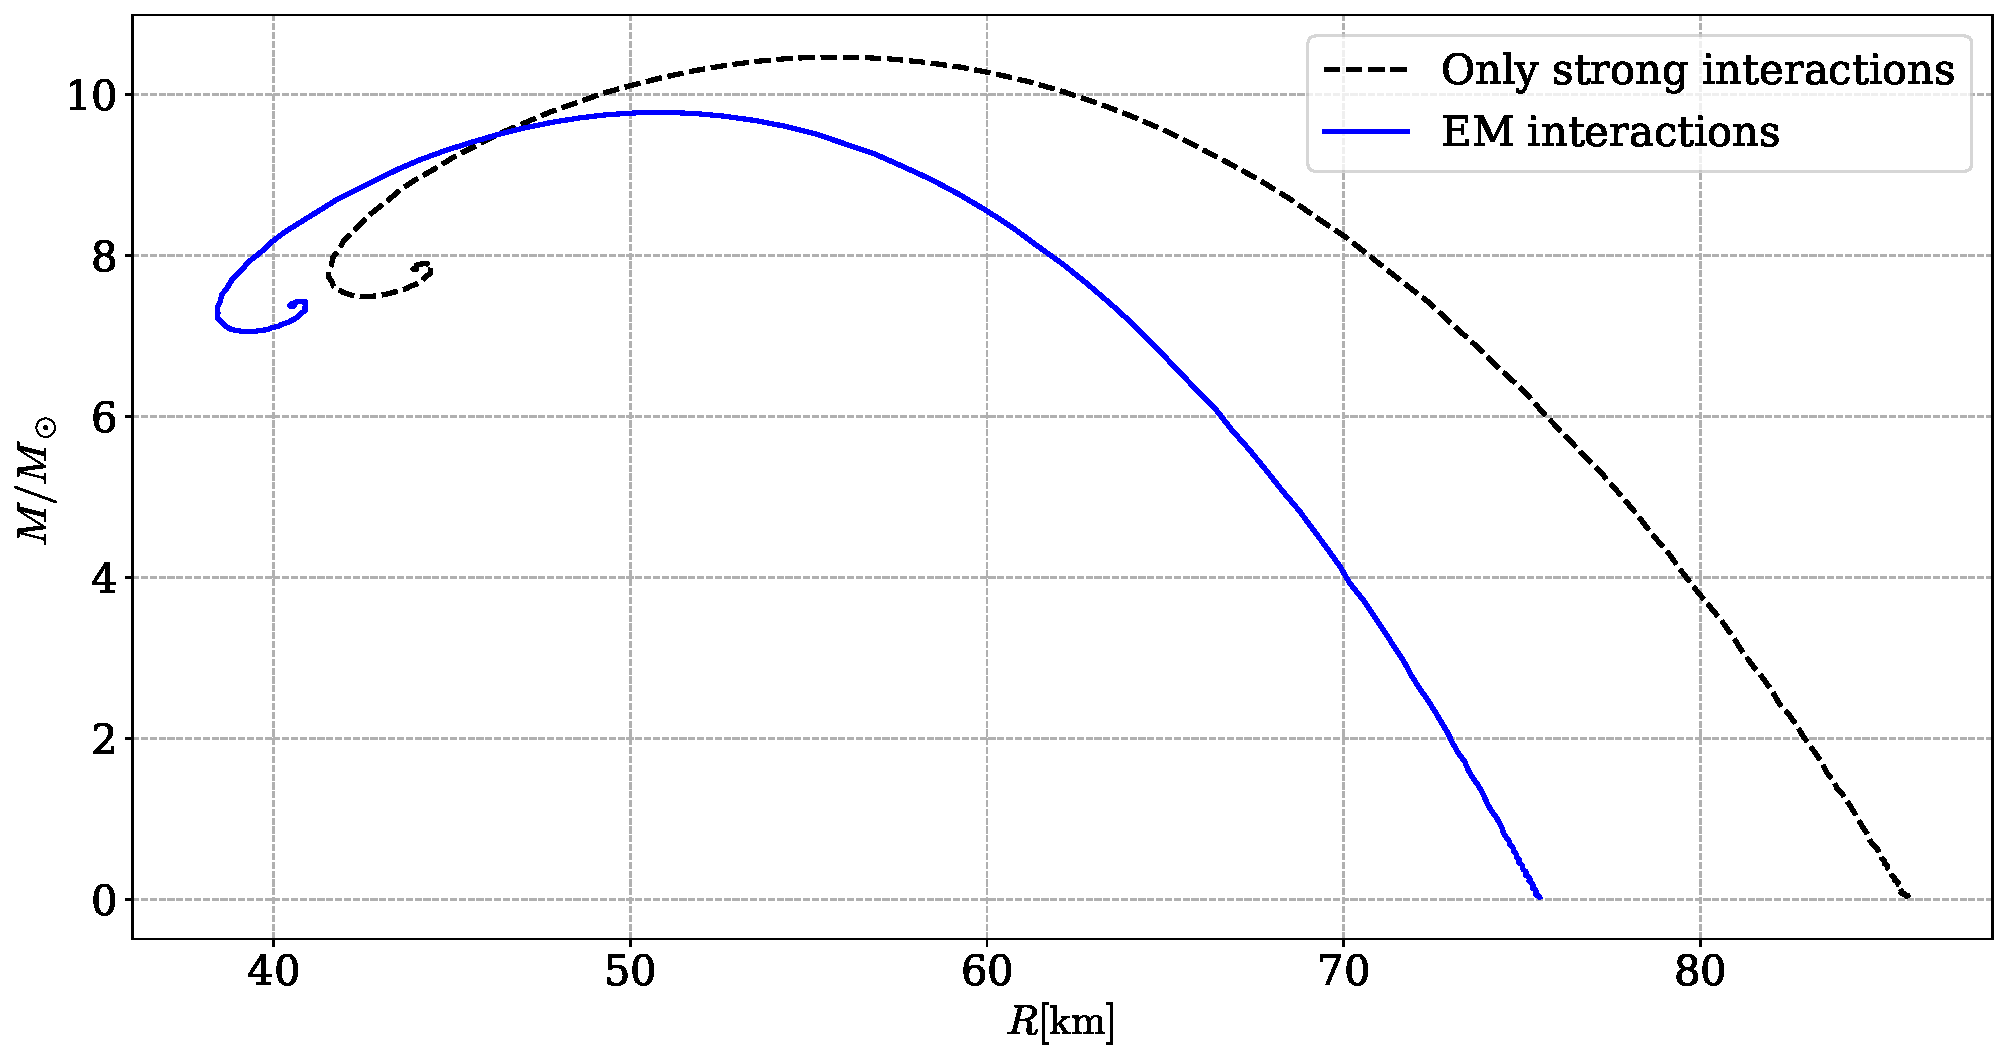
\includegraphics[width=\textwidth]{../../scripts/figurer/pion_star/mass_radius_pion_star_compare.pdf}
    \end{frame}

    \begin{frame}
        \frametitle{Limit}
        
        \begin{textblock}{9}(6.8, 1)
            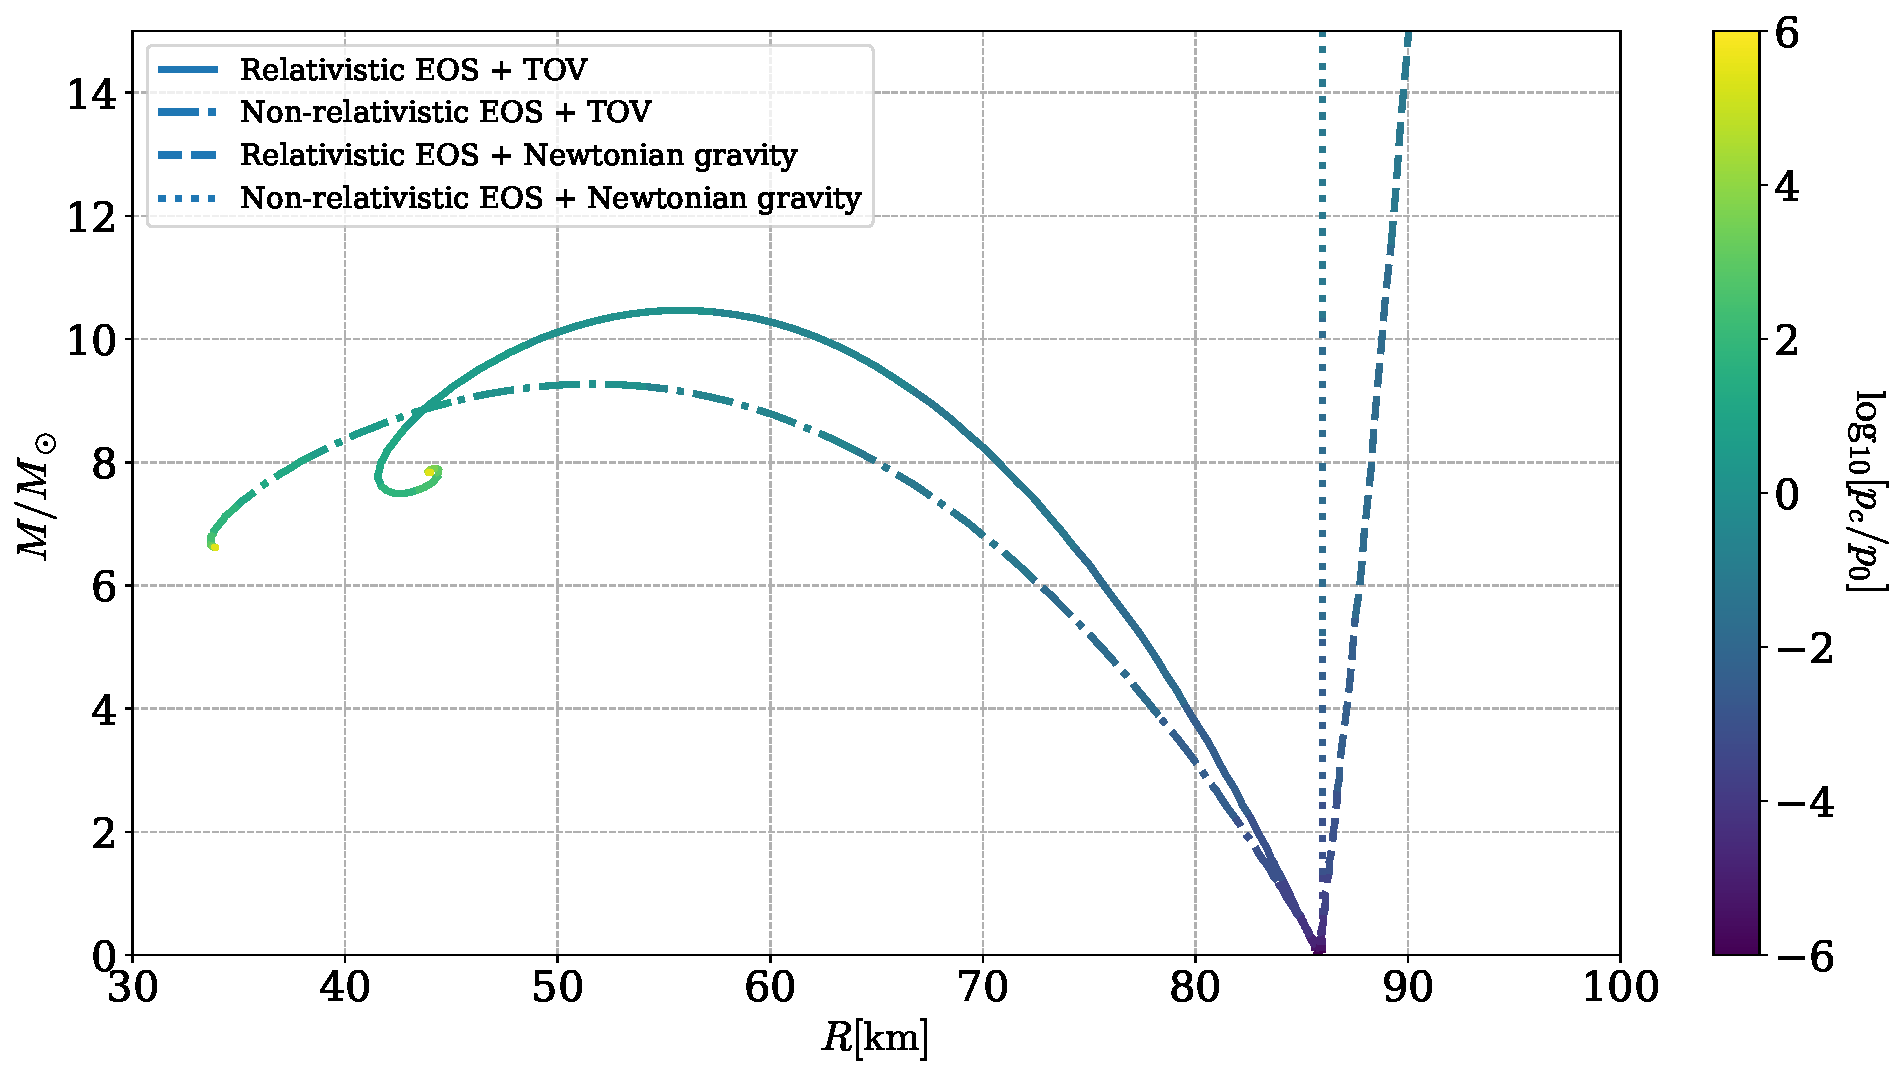
\includegraphics[width=\textwidth]{../../scripts/figurer/pion_star/mass_radius_comparison.pdf}
        \end{textblock}

        \begin{itemize}
            \itemsep 0.4cm
            \item Newtonian and non-relativistic \\ limit of EOS and TOV
            \item Used to derive Chandrasekhar \\ limit
            \item Non-relativistic limit of pion \\ equation of state is polytrope,\\ $P = Ku^2$
            \item We can show that radius is independent of external pressure, and $R = \frac{\pi r^0}{\sqrt{12}}$.
        \end{itemize}

    \end{frame}


\end{document}
